% Options for packages loaded elsewhere
\PassOptionsToPackage{unicode}{hyperref}
\PassOptionsToPackage{hyphens}{url}
%
\documentclass[
]{article}
\usepackage{lmodern}
\usepackage{amssymb,amsmath}
\usepackage{ifxetex,ifluatex}
\ifnum 0\ifxetex 1\fi\ifluatex 1\fi=0 % if pdftex
  \usepackage[T1]{fontenc}
  \usepackage[utf8]{inputenc}
  \usepackage{textcomp} % provide euro and other symbols
\else % if luatex or xetex
  \usepackage{unicode-math}
  \defaultfontfeatures{Scale=MatchLowercase}
  \defaultfontfeatures[\rmfamily]{Ligatures=TeX,Scale=1}
\fi
% Use upquote if available, for straight quotes in verbatim environments
\IfFileExists{upquote.sty}{\usepackage{upquote}}{}
\IfFileExists{microtype.sty}{% use microtype if available
  \usepackage[]{microtype}
  \UseMicrotypeSet[protrusion]{basicmath} % disable protrusion for tt fonts
}{}
\makeatletter
\@ifundefined{KOMAClassName}{% if non-KOMA class
  \IfFileExists{parskip.sty}{%
    \usepackage{parskip}
  }{% else
    \setlength{\parindent}{0pt}
    \setlength{\parskip}{6pt plus 2pt minus 1pt}}
}{% if KOMA class
  \KOMAoptions{parskip=half}}
\makeatother
\usepackage{xcolor}
\IfFileExists{xurl.sty}{\usepackage{xurl}}{} % add URL line breaks if available
\IfFileExists{bookmark.sty}{\usepackage{bookmark}}{\usepackage{hyperref}}
\hypersetup{
  hidelinks,
  pdfcreator={LaTeX via pandoc}}
\urlstyle{same} % disable monospaced font for URLs
\usepackage{color}
\usepackage{fancyvrb}
\newcommand{\VerbBar}{|}
\newcommand{\VERB}{\Verb[commandchars=\\\{\}]}
\DefineVerbatimEnvironment{Highlighting}{Verbatim}{commandchars=\\\{\}}
% Add ',fontsize=\small' for more characters per line
\newenvironment{Shaded}{}{}
\newcommand{\AlertTok}[1]{\textcolor[rgb]{1.00,0.00,0.00}{\textbf{#1}}}
\newcommand{\AnnotationTok}[1]{\textcolor[rgb]{0.38,0.63,0.69}{\textbf{\textit{#1}}}}
\newcommand{\AttributeTok}[1]{\textcolor[rgb]{0.49,0.56,0.16}{#1}}
\newcommand{\BaseNTok}[1]{\textcolor[rgb]{0.25,0.63,0.44}{#1}}
\newcommand{\BuiltInTok}[1]{#1}
\newcommand{\CharTok}[1]{\textcolor[rgb]{0.25,0.44,0.63}{#1}}
\newcommand{\CommentTok}[1]{\textcolor[rgb]{0.38,0.63,0.69}{\textit{#1}}}
\newcommand{\CommentVarTok}[1]{\textcolor[rgb]{0.38,0.63,0.69}{\textbf{\textit{#1}}}}
\newcommand{\ConstantTok}[1]{\textcolor[rgb]{0.53,0.00,0.00}{#1}}
\newcommand{\ControlFlowTok}[1]{\textcolor[rgb]{0.00,0.44,0.13}{\textbf{#1}}}
\newcommand{\DataTypeTok}[1]{\textcolor[rgb]{0.56,0.13,0.00}{#1}}
\newcommand{\DecValTok}[1]{\textcolor[rgb]{0.25,0.63,0.44}{#1}}
\newcommand{\DocumentationTok}[1]{\textcolor[rgb]{0.73,0.13,0.13}{\textit{#1}}}
\newcommand{\ErrorTok}[1]{\textcolor[rgb]{1.00,0.00,0.00}{\textbf{#1}}}
\newcommand{\ExtensionTok}[1]{#1}
\newcommand{\FloatTok}[1]{\textcolor[rgb]{0.25,0.63,0.44}{#1}}
\newcommand{\FunctionTok}[1]{\textcolor[rgb]{0.02,0.16,0.49}{#1}}
\newcommand{\ImportTok}[1]{#1}
\newcommand{\InformationTok}[1]{\textcolor[rgb]{0.38,0.63,0.69}{\textbf{\textit{#1}}}}
\newcommand{\KeywordTok}[1]{\textcolor[rgb]{0.00,0.44,0.13}{\textbf{#1}}}
\newcommand{\NormalTok}[1]{#1}
\newcommand{\OperatorTok}[1]{\textcolor[rgb]{0.40,0.40,0.40}{#1}}
\newcommand{\OtherTok}[1]{\textcolor[rgb]{0.00,0.44,0.13}{#1}}
\newcommand{\PreprocessorTok}[1]{\textcolor[rgb]{0.74,0.48,0.00}{#1}}
\newcommand{\RegionMarkerTok}[1]{#1}
\newcommand{\SpecialCharTok}[1]{\textcolor[rgb]{0.25,0.44,0.63}{#1}}
\newcommand{\SpecialStringTok}[1]{\textcolor[rgb]{0.73,0.40,0.53}{#1}}
\newcommand{\StringTok}[1]{\textcolor[rgb]{0.25,0.44,0.63}{#1}}
\newcommand{\VariableTok}[1]{\textcolor[rgb]{0.10,0.09,0.49}{#1}}
\newcommand{\VerbatimStringTok}[1]{\textcolor[rgb]{0.25,0.44,0.63}{#1}}
\newcommand{\WarningTok}[1]{\textcolor[rgb]{0.38,0.63,0.69}{\textbf{\textit{#1}}}}
\usepackage{graphicx}
\makeatletter
\def\maxwidth{\ifdim\Gin@nat@width>\linewidth\linewidth\else\Gin@nat@width\fi}
\def\maxheight{\ifdim\Gin@nat@height>\textheight\textheight\else\Gin@nat@height\fi}
\makeatother
% Scale images if necessary, so that they will not overflow the page
% margins by default, and it is still possible to overwrite the defaults
% using explicit options in \includegraphics[width, height, ...]{}
\setkeys{Gin}{width=\maxwidth,height=\maxheight,keepaspectratio}
% Set default figure placement to htbp
\makeatletter
\def\fps@figure{htbp}
\makeatother
\setlength{\emergencystretch}{3em} % prevent overfull lines
\providecommand{\tightlist}{%
  \setlength{\itemsep}{0pt}\setlength{\parskip}{0pt}}
\setcounter{secnumdepth}{-\maxdimen} % remove section numbering

\author{}
\date{}

\documentclass[a4paper,11pt]{proc}
\usepackage[a4paper,margin=2cm,footskip=1cm]{geometry}
\usepackage[utf8]{inputenc}
\usepackage{fancyhdr}
\usepackage{graphicx}
\usepackage{listings}
\usepackage{xcolor}
\usepackage[hidelinks]{hyperref}
\usepackage{textcomp}
\usepackage[section]{placeins}
\usepackage[T1]{fontenc}

\definecolor{codegreen}{rgb}{0,0.6,0}
\definecolor{codegray}{rgb}{0.5,0.5,0.5}
\definecolor{codepurple}{rgb}{0.58,0,0.82}
\definecolor{backcolour}{rgb}{0.95,0.95,0.92}
\definecolor{codepurple}{HTML}{C42043}
\definecolor{backcolour}{HTML}{F2F2F2}
\definecolor{bookColor}{cmyk}{0,0,0,0.90}  
\color{bookColor}

\lstset{upquote=true}

\lstloadlanguages{C,C++,csh,Java}

\lstdefinestyle{mystyle}{
	backgroundcolor=\color{backcolour},   
	commentstyle=\color{codegreen},
	keywordstyle=\color{codepurple},
	numberstyle=\footnotesize\color{codegray},
	stringstyle=\color{codepurple},
	basicstyle=\footnotesize,
	breakatwhitespace=false,         
	breaklines=true,                 
	captionpos=b,                    
	keepspaces=true,                 
	numbers=left,                    
	numbersep=10pt,                  
	showspaces=false,                
	showstringspaces=false,
	showtabs=false,      
}
\lstset{style=mystyle} 

\pagestyle{fancy}
\title{Approximating Roots with Computation}
\author{Rushil Ambati}

\rhead{Approximating Roots with Computation}
\lfoot{Rushil Ambati}

\begin{document}
%----------------------------------------------------------------------------------------
%	TITLE PAGE
%----------------------------------------------------------------------------------------

\begin{titlepage} % Suppresses displaying the page number on the title page and the subsequent page counts as page 1
	
	\raggedleft % Right align the title page
	
	\rule{1pt}{\textheight} % Vertical line
	\hspace{0.05\textwidth} % Whitespace between the vertical line and title page text
	\parbox[b]{0.75\textwidth}{ % Paragraph box for holding the title page text, adjust the width to move the title page left or right on the page
		
		{\Huge\bfseries Approximating Roots \\[0.5\baselineskip] with Computation}\\[2\baselineskip] % Title
		{\large\textit{A mini-project}}\\[4\baselineskip] % Subtitle or further description
		{\Large\textsc{Rushil Ambati}} % Author name, lower case for consistent small caps
		
		\vspace{0.5\textheight} % Whitespace between the title block and the publisher

	}

\end{titlepage}

%----------------------------------------------------------------------------------------
\hypertarget{header-n4}{%
\subsection{Outline}\label{header-n4}}

In this mini-project I'll be using numerical methods and computation in
order to approximate roots of an equation.

The specific method used here is called the \emph{Newton-Raphson method}
(alternatively known as just `\emph{Newton's method}'), named after
Isaac Newton and Joseph Raphson.

\tableofcontents
\newpage


\hypertarget{header-n8}{%
\subsection{Theory}\label{header-n8}}

\hypertarget{header-n9}{%
\subsubsection{Newton-Raphson method}\label{header-n9}}

\begin{quote}
For a single-variable function \(f\) defined for a real variable \(x\)
with derivative \(f'\) and an initial guess \(x_0\) for a root of \(f\).
If the function satisfies assumptions, and the initial guess is close,
then

\[x_1 = x_0 - \frac{f(x_0)}{f'(x_0)}\]

where \(x_1\) is a better approximation of the root than \(x_0\).
Geometrically, \((x_1, 0)\) is the intersection of the x-axis and the
tangent of the graph of f at \((x_0, f(x0))\): that is, the improved
guess is the unique root of the linear approximation at the initial
point. The process is repeated as

\[x_{n+1} = x_n - \frac{f(x_n)}{f'(x_n)}\]

until a sufficiently precise value is reached. This algorithm is first
in the class of Householder's methods, succeeded by Halley's method. The
method can also be extended to complex functions and to systems of
equations.

(\href{https://en.wikipedia.org/wiki/Newton's_method}{\emph{Source}})
\end{quote}

\hypertarget{header-n18}{%
\subsubsection{Derivation of the equation}\label{header-n18}}

The iterative equation \(x_{n+1} = x_n - \frac{f(x_n)}{f'(x_n)}\) is the
form in the A-level specification too, and we'll use the same in our
program here.\\
However, we weren't taught the derivation in class, so I'll attempt one
here.

The geometric description above can be represented in a graph diagram,
such as the one below:
\begin{figure}
\centering
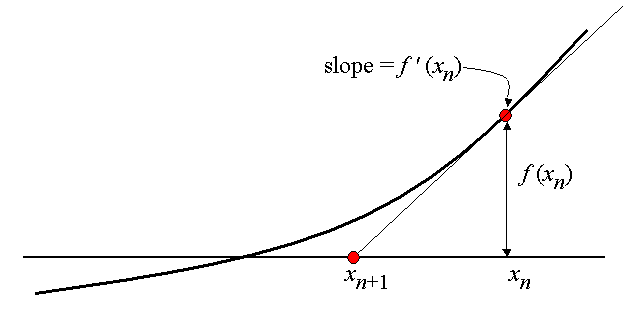
\includegraphics[width=0.7\columnwidth]{./diagram_1.png}
(\href{https://brilliant.org/wiki/newton-raphson-method/}{\emph{Source}})
\end{figure}

So we now have a tangent at \(x_n\) that has the following
characteristics:

\begin{itemize}
\item
  It goes through the point \((x_n, f(x_n))\)
\item
  It has gradient \(f'(x_n)\)
\end{itemize}

So now to get the equation of the tangent, we can put it into point
slope form \(y-y_1=m(x-x_1)\):

\[y-f(x_n)=f'(x_n)(x-x_n)\]

We want our value of \(x\) when \(y=0\) (or the root of the equation):

\[f(x_n)+f'(x_n)(x-x_n)=0\]

Hence if we solve for \(x\), which will be the x-intercept and closer to
the root (our \(x_{n+1}\)):

\[f'(x_n)(x-x_n)=-f(x_n)\]
\[x-x_n=-\frac{f(x_n)}{f'(x_n)}\]
\[x=x_n-\frac{f(x_n)}{f'(x_n)}\]

we obtain our desired form.

\hypertarget{header-n38}{%
\subsubsection{Limitations and Practical
Considerations}\label{header-n38}}

\begin{quote}
\mbox{}%
\hypertarget{header-n40}{%
\paragraph{Difficulty in calculating the derivative of a
function}\label{header-n40}}
\hfill \break
Newton's method requires that the derivative can be calculated directly.
An analytical expression for the derivative may not be easily obtainable
or could be expensive to evaluate. In these situations, it may be
appropriate to approximate the derivative by using the slope of a line
through two nearby points on the function. Using this approximation
would result in something like the \emph{secant method} whose
convergence is slower than that of Newton's method.

\hypertarget{header-n42}{%
\paragraph{Overshoot}\label{header-n42}}
\hfill \break
If the first derivative is not well behaved in the neighbourhood of a
particular root, the method may overshoot, and diverge from that root.
This includes points of inflection, local maxima or minima around
\(x_0\) or the root.

\hypertarget{header-n44}{%
\paragraph{Features of graph around root}\label{header-n44}}
\hfill \break
If a stationary point of the function is encountered, the derivative is
zero and the method will terminate due to division by zero.

\hypertarget{header-n46}{%
\paragraph{Poor initial estimate}\label{header-n46}}
\hfill \break
A large error in the initial estimate can contribute to non-convergence
of the algorithm.

\hypertarget{header-n48}{%
\paragraph{Discontinuity}\label{header-n48}}
\hfill \break
This will only work for functions defined for all real numbers.
Asymptotes will also yield undefined values.

(\href{https://en.wikipedia.org/wiki/Newton\%27s_method\#Failure_of_the_method_to_converge_to_the_root}{\emph{Source}})
\end{quote}

\hypertarget{header-n52}{%
\subsection{Implementation}\label{header-n52}}

\hypertarget{header-n53}{%
\subsubsection{Newton-Raphson Method}\label{header-n53}}

Firstly, we'll define our function. Let's say for the sake of our
example we're trying to find the roots of \(x^2-4x-7=0\).

\begin{Shaded}
\begin{Highlighting}[]
\KeywordTok{def}\NormalTok{ f(x):}
    \ControlFlowTok{return}\NormalTok{ (x}\OperatorTok{**}\DecValTok{2}\OperatorTok{{-}}\DecValTok{4}\OperatorTok{*}\NormalTok{x}\OperatorTok{{-}}\DecValTok{7}\NormalTok{)}
\end{Highlighting}
\end{Shaded}

Next, we'll define the derivative of our function (so we can use it in
place of the \(f'(x_n)\) in the equation).

\begin{Shaded}
\begin{Highlighting}[]
\KeywordTok{def}\NormalTok{ f\_prime(x):}
    \ControlFlowTok{return} \DecValTok{2}\OperatorTok{*}\NormalTok{x}\OperatorTok{{-}}\DecValTok{4}
\end{Highlighting}
\end{Shaded}

Now we've got all our setup done, let's construct a function that will
actually carry out the Newton-Raphson method.

\begin{Shaded}
\begin{Highlighting}[]
\KeywordTok{def}\NormalTok{ nrf(guess, n):}
    \BuiltInTok{print}\NormalTok{(}\StringTok{"x\_0 = "} \OperatorTok{+} \BuiltInTok{str}\NormalTok{(guess))}
    \ControlFlowTok{for}\NormalTok{ i }\KeywordTok{in} \BuiltInTok{range}\NormalTok{(n}\OperatorTok{+}\DecValTok{1}\NormalTok{):}
\NormalTok{        next\_guess }\OperatorTok{=}\NormalTok{ guess }\OperatorTok{{-}}\NormalTok{ f(guess) }\OperatorTok{/}\NormalTok{ f\_prime(guess)}
        \BuiltInTok{print}\NormalTok{(}\StringTok{"x\_"} \OperatorTok{+} \BuiltInTok{str}\NormalTok{(i}\OperatorTok{+}\DecValTok{1}\NormalTok{) }\OperatorTok{+} \StringTok{" = "} \OperatorTok{+} \BuiltInTok{str}\NormalTok{(next\_guess))}
\NormalTok{        guess }\OperatorTok{=}\NormalTok{ next\_guess}
\end{Highlighting}
\end{Shaded}

Now, let's call it. Say our starting value is 8, and we want it to
iterate 10 times.

\begin{Shaded}
\begin{Highlighting}[]
\NormalTok{nrf(}\DecValTok{8}\NormalTok{, }\DecValTok{10}\NormalTok{)}
\end{Highlighting}
\end{Shaded}

This provides the following output:

\begin{Shaded}
\begin{Highlighting}[]
\NormalTok{x\_0 = }\DecValTok{8}
\NormalTok{x\_1 = }\DecValTok{5}\NormalTok{.916666666666666}
\NormalTok{x\_2 = }\DecValTok{5}\NormalTok{.36258865248227}
\NormalTok{x\_3 = }\DecValTok{5}\NormalTok{.316938934730458}
\NormalTok{x\_4 = }\DecValTok{5}\NormalTok{.316624805231569}
\NormalTok{x\_5 = }\DecValTok{5}\NormalTok{.3166247903554}
\NormalTok{x\_6 = }\DecValTok{5}\NormalTok{.3166247903554}
\NormalTok{x\_7 = }\DecValTok{5}\NormalTok{.3166247903554}
\NormalTok{x\_8 = }\DecValTok{5}\NormalTok{.3166247903554}
\NormalTok{x\_9 = }\DecValTok{5}\NormalTok{.3166247903554}
\NormalTok{x\_10 = }\DecValTok{5}\NormalTok{.3166247903554}
\end{Highlighting}
\end{Shaded}

So our final value for the root closest to 8 is approximately 5.32 (to 3
significant figures.)\\
The true value of that positive root is \(2+\sqrt{11}\) and our
approximation of 5.3166\ldots{} is actually very close, and didn't take
that many iterations to reach there. This is because our starting value
of 8 is very close to the actual root.

We can also find the other root of this quadratic equation by starting
at another value, say -4, iterating the same number of times.

\begin{Shaded}
\begin{Highlighting}[]
\NormalTok{nrf(}\OperatorTok{{-}}\DecValTok{4}\NormalTok{, }\DecValTok{10}\NormalTok{)}
\end{Highlighting}
\end{Shaded}

This provides the following output:

\begin{verbatim}
x_0 = -4
x_1 = -1.9166666666666665
x_2 = -1.3625886524822695
x_3 = -1.3169389347304572
x_4 = -1.3166248052315688
x_5 = -1.3166247903553998
x_6 = -1.3166247903553998
x_7 = -1.3166247903553998
x_8 = -1.3166247903553998
x_9 = -1.3166247903553998
x_10 = -1.3166247903553998
\end{verbatim}

The other root is \(2-\sqrt{11}\) and our approximate of -1.3166\ldots{}
is also close. It reached a static value in just 5 iterations.

\hypertarget{header-n71}{%
\subsubsection{Secant Method - Tackling the derivative
problem}\label{header-n71}}

\hypertarget{header-n72}{%
\paragraph{Theory}\label{header-n72}}
\hfill \break
In the \protect\hyperlink{header-n38}{Limitations and Practical
Considerations}, we considered the possibility that we could be working
with a function that may not have an easily obtainable derivative. In
this case, I'll work around this problem by using an alternative method
called the \emph{Secant Method}. Although different in name, the only
main difference between the \emph{Newton-Raphson method} and the
\emph{Secant method} is the way that \(f'(x_n)\) is calculated.

Instead of using an expression to programatically write in the
derivative of the function, eg. \texttt{x**2-4*x-7}`s derivative being
\texttt{2*x-4} we will use a finite difference method to calculate the
derivative at a point of \(f(x)\). The `quotient difference', on which
this method relies on, is nothing more than the fundamental idea that
differentiation relies on.

We take differentiation from first principles to be as such:

\[f'(x)=\lim_{x\to0}\frac{f(x+h)-f(x)}{h}\]

So, if we use a small value of \(h\) and just use our function for
\(f(x)\) we can get an approximation for the value of \(f'(x)\) for any
\(x\). This means we don't actually have to evaluate the expression for
the derivative, providing a workaround for the limitation discussed
above.

\hypertarget{header-n78}{%
\paragraph{Implementation}\label{header-n78}}
\hfill \break
All we have to do now, is to change our \texttt{f\_prime} function to
compute the quotient difference at some \(x\) with some difference value
\(h\).

\begin{Shaded}
\begin{Highlighting}[]
\KeywordTok{def}\NormalTok{ f\_prime(x, h):}
    \ControlFlowTok{return}\NormalTok{ (f(x }\OperatorTok{+}\NormalTok{ h) }\OperatorTok{{-}}\NormalTok{ f(x)) }\OperatorTok{/}\NormalTok{ h}
\end{Highlighting}
\end{Shaded}

Of course, the smaller our \(h\) is, the better the approximation for
the derivative, but the more expensive it is computationally.

\hypertarget{header-n83}{%
\subsection{Final Code}\label{header-n83}}

\begin{Shaded}
\begin{Highlighting}[]
\KeywordTok{def}\NormalTok{ f(x):}
    \CommentTok{\# Define your function here}
    \ControlFlowTok{return}\NormalTok{ (x}\OperatorTok{**}\DecValTok{2}\OperatorTok{{-}}\DecValTok{4}\OperatorTok{*}\NormalTok{x}\OperatorTok{{-}}\DecValTok{7}\NormalTok{)}

\KeywordTok{def}\NormalTok{ f\_prime(x):}
    \CommentTok{\# Define your function\textquotesingle{}s first derivative here}
    \ControlFlowTok{return} \DecValTok{2}\OperatorTok{*}\NormalTok{x}\OperatorTok{{-}}\DecValTok{4}

\KeywordTok{def}\NormalTok{ f\_prime\_sec(x, h):}
    \CommentTok{"""Calculates the value of the derivative of a function }

\CommentTok{    Args:}
\CommentTok{        x (float): The value for which we are calculating the derivative value}
\CommentTok{        h (float): Quotient difference}

\CommentTok{    Returns:}
\CommentTok{        float: Approximate derivative of f(x) at x, with quotient difference h}
\CommentTok{    """}
    \ControlFlowTok{return}\NormalTok{ (f(x }\OperatorTok{+}\NormalTok{ h) }\OperatorTok{{-}}\NormalTok{ f(x)) }\OperatorTok{/}\NormalTok{ h}
    
\KeywordTok{def}\NormalTok{ approximate\_root(guess, n, sec}\OperatorTok{=}\VariableTok{False}\NormalTok{, h}\OperatorTok{=}\DecValTok{1}\OperatorTok{*}\DecValTok{10}\OperatorTok{**{-}}\DecValTok{3}\NormalTok{):}
    \CommentTok{"""Iteratively estimates the roots of a function by using the Newton{-}Raphson Method}

\CommentTok{    Args:}
\CommentTok{        guess (float): Initial value to iterate from}
\CommentTok{        n (int): Number of iterations}
\CommentTok{        sec (bool, optional): Whether or not to use the secant method. Defaults to False.}
\CommentTok{        h (float, optional): Quotient difference interval. Defaults to 1x10\^{}{-}3.}
\CommentTok{    """}
    \BuiltInTok{print}\NormalTok{(}\StringTok{"x\_0 = "} \OperatorTok{+} \BuiltInTok{str}\NormalTok{(guess))}
    \ControlFlowTok{for}\NormalTok{ i }\KeywordTok{in} \BuiltInTok{range}\NormalTok{(n):}
\NormalTok{        f\_prime\_x }\OperatorTok{=}\NormalTok{ f\_prime\_sec(guess, h) }\ControlFlowTok{if}\NormalTok{ (sec }\OperatorTok{==} \VariableTok{True}\NormalTok{) }\ControlFlowTok{else}\NormalTok{ f\_prime(guess)}
\NormalTok{        next\_guess }\OperatorTok{=}\NormalTok{ guess }\OperatorTok{{-}}\NormalTok{ f(guess) }\OperatorTok{/}\NormalTok{ f\_prime\_x }\CommentTok{\# Evaluating x\_n+1}
        \BuiltInTok{print}\NormalTok{(}\StringTok{"x\_"} \OperatorTok{+} \BuiltInTok{str}\NormalTok{(i}\OperatorTok{+}\DecValTok{1}\NormalTok{) }\OperatorTok{+} \StringTok{" = "} \OperatorTok{+} \BuiltInTok{str}\NormalTok{(next\_guess))}
\NormalTok{        guess }\OperatorTok{=}\NormalTok{ next\_guess}
\end{Highlighting}
\end{Shaded}

Function can be invoked as follows:

\begin{Shaded}
\begin{Highlighting}[]
\NormalTok{approximate\_root(}\DecValTok{8}\NormalTok{, }\DecValTok{10}\NormalTok{) }\CommentTok{\# Uses the derivative manually calculated}
\NormalTok{approximate\_root(}\OperatorTok{{-}}\DecValTok{4}\NormalTok{, }\DecValTok{10}\NormalTok{, sec}\OperatorTok{=}\VariableTok{True}\NormalTok{) }\CommentTok{\# Uses secant method to approximate derivative}
\end{Highlighting}
\end{Shaded}
\newpage
\hypertarget{header-n88}{%
\subsection{Points for discussion}\label{header-n88}}

\begin{itemize}
\item
  To see how the Secant method compares to the Newton-Raphson method
  depending on the type of graph considered or other factors.
\item
  To look into other numerical methods that have other use-cases, as
  well as how they compare to the two considered above.
\item
  I wonder if there's a more efficient way to write up my algorithm.
  Also, this is a simple enough algorithm, and doesn't use any libraries
  so isn't difficult to port to other languages. Maybe try porting it to
  something like C, where it'd actually be somewhat efficient - who
  knows, maybe even in Assembly?
\item
  It'd be cool to see both of these methods applied to:

  \begin{itemize}
  \item
    More than one dimension.
  \item
    Complex functions
  \item
    Systems of equations
  \end{itemize}
\item
  If it's possible (in some, or even all cases) to mathematically prove
  whether or not the iterative method will converge given a particular
  starting value and the equation of the graph.
\item
  I've heard about the `Laplace Transform' when talking about numerical
  methods, I wonder what that is.
\item
  On the Wikipedia page for the Secant method, it discusses the ``order
  of convergence'' and the golden ratio. It'd be interesting to see
  where the golden ratio fits into it all.

  \begin{quote}
  The iterates \(x_n\) of the secant method converge to a root of \(f\),
  if the initial values \(x_0\) and \(x_1\) are sufficiently close to
  the root. The order of convergence is \(\varphi\), where

  \[\varphi=\frac{1+\sqrt{5}}{2}\approx1.618\]

  is the golden ratio. In particular, the convergence is superlinear,
  but not quite quadratic.

  This result only holds under some technical conditions, namely that
  \(f\) be twice continuously differentiable and the root in question be
  simple (i.e., with multiplicity 1).

  (\href{https://en.wikipedia.org/wiki/Secant_method\#Convergence}{\emph{Source}})
  \end{quote}
\end{itemize}

\end{document}
